% learned_sigma_profile.tex -- перезаписанная рукопись. Компилируется XeLaTeX, дважды.
% Прежний файл grounding_paradox.tex сохранён как есть: это другая рамка, не редакция этой.
% ВЁРСТКА. layout=twocolumn даёт журнальный вид, 14 страниц; layout=traditional -- формат
% подачи ACS (одна колонка, двойной интервал), те же 4700 слов тела занимают там 25 страниц.
% Объём содержания от переключателя не зависит; менять его для сдачи, а не для счёта страниц.
\documentclass[journal=jcisd8,manuscript=article,layout=twocolumn]{achemso}
% =====================================================================
% SHARED PREAMBLE, \input by BOTH documents of this submission:
%   grounding_paradox.tex      the article                (manuscript=article)
%   grounding_paradox_si.tex   the Supporting Information (manuscript=suppinfo)
% Split out on 2026-08-02, when the Supporting Information became its own file at
% the request of all three referees and because ACS deposits it as a separate one.
% Everything here was the article's own preamble before the split and is unchanged
% apart from the xr-hyper line; the point of the file is that the two documents
% cannot drift apart -- a macro added for one is defined for both.
% What is NOT here, because it differs between the two: \documentclass (the
% manuscript type), the title/author/abstract block, \abbreviations, \keywords,
% \externaldocument (each document names the other), and the Supporting
% Information's S-numbering.
% =====================================================================
\SectionNumbersOn
\usepackage{amsmath,amssymb,amsthm}
\usepackage{array}
\usepackage{booktabs}
% Ragged-right paragraph column. Narrow justified p-columns in the claim and
% decomposition tables stretched a two-word line across the whole column; L{} sets the
% same text without the stretch, which is what let the column widths be rebalanced
% against actual content instead of against the worst justified line.
\newcolumntype{L}[1]{>{\raggedright\arraybackslash}p{#1}}
\usepackage{graphicx}
\usepackage{xcolor}
% ---------------------------------------------------------------------
% CROSS-DOCUMENT REFERENCES. The article and the Supporting Information are two
% separate documents, so neither LaTeX run can see the other's \label{}s. xr-hyper
% reads the other document's .aux and makes its labels resolve to the ordinary
% \ref, so not one of the 234 references that cross the boundary had to be rewritten
% as a hand-maintained plain-text pointer. The Supporting Information numbers itself
% S1, S2, ... (sections, tables, figures, equations, lemmas), so a resolved number
% says by itself which of the two documents it is in.
% xr-hyper, NOT xr: under hyperref \newlabel carries five arguments and plain xr
% reads the wrong one. It has to be loaded BEFORE hyperref, which is the only reason
% this line sits here and not beside \externaldocument.
% BUILD ORDER follows from it: the first pass of either document writes the .aux the
% other one reads, so from a clean directory it is xelatex on both, bibtex on both,
% then xelatex on both twice more. Building only one of the two from clean leaves
% its cross-document references as `??', and LaTeX reports that as a warning, not an
% error -- check the log for "There were undefined references", do not trust the
% exit status alone.
% ---------------------------------------------------------------------
\usepackage{xr-hyper}
% hidelinks: without it hyperref's default pdfborder={0 0 1} draws a rectangle around every
% cross-reference and citation. The boxes are invisible on screen in some viewers but print,
% and ACS production receives the PDF as-is.
\usepackage[hidelinks]{hyperref}

% ---------------------------------------------------------------------
% FLOAT PLACEMENT. In the two-column measure a deferred `table*'/`figure*' blocks every
% starred float after it, and stock LaTeX flushes that queue only at \clearpage -- which
% here is \end{document}. Left alone, every float from Table 2 onward printed after the
% bibliography, tens of pages from the text that cites it. dblfloatfix repairs the ordering
% and lets a double float reach the bottom of a column; the fractions below let a tall
% starred float be a top float instead of being sent to a float page. The starred floats that sit
% at that height limit additionally carry `p' in their own placement specifiers, so a float page is
% available to them and the queue never backs up; the note at each of them says so. Give a new tall
% `table*'/`figure*' the same `p'. Do NOT name those floats by number here: the numbering has moved
% twice as tables crossed between the two documents, and a stale number in this comment sends the
% next reader to the wrong float. Do NOT force the queue out with \afterpage{\clearpage} before Sec. 6.5
% or before the Discussion: in two-column mode that fires at a column boundary rather than a
% page boundary, so it ends the page with the right-hand column empty -- a blank half page
% before the Discussion -- and it buys no placement that `p' does not.
% Do not tighten these back without checking where the floats land.
% ---------------------------------------------------------------------
\usepackage{dblfloatfix}
\renewcommand{\topfraction}{0.92}
\renewcommand{\dbltopfraction}{0.92}
\renewcommand{\bottomfraction}{0.6}
\renewcommand{\textfraction}{0.06}
\renewcommand{\floatpagefraction}{0.6}
\renewcommand{\dblfloatpagefraction}{0.6}
\setcounter{topnumber}{3}
\setcounter{dbltopnumber}{3}
\setcounter{bottomnumber}{2}
\setcounter{totalnumber}{5}

\newtheorem{theorem}{Theorem}
\newtheorem{lemma}{Lemma}
\newtheorem{proposition}{Proposition}
\newtheorem{corollary}{Corollary}
\newtheorem{assumption}{Assumption}
\newtheorem{definition}{Definition}

% amsthm sets the optional argument of `proof' as a \trivlist label, i.e. one unbreakable
% \hbox. Four of the SI proof headers are longer than the two-column measure and ran into the
% neighbouring column. This redefinition is amsthm's own, with the head moved out of the label
% and into the paragraph so it wraps; \pushQED/\popQED and the spacing are unchanged.
\makeatletter
\renewenvironment{proof}[1][\proofname]{\par
  \pushQED{\qed}%
  \normalfont \topsep6\p@\@plus6\p@\relax
  \trivlist
  \item[]\hskip\labelsep{\itshape #1\@addpunct{.}}\enspace\ignorespaces
}{\popQED\endtrivlist\@endpefalse}
\makeatother

% ---------------------------------------------------------------------
% ACS-style lettered table footnotes. \tnk{a} sets the superscript key in the row or
% column head it qualifies; \tabnotes{...} sets the note block directly under the
% \bottomrule. THIS IS THE DESTINATION FOR CAPTION MATERIAL. A caption says what the
% table shows; anything that qualifies one row, one column or one cell is keyed to it
% here instead of being appended to the caption. Budget: <=40 words for a table
% caption, <=60 for a figure caption. Captions on this manuscript have been cut twice
% and grown back twice because each repair pass appended a sentence; if a finding
% needs an answer, put the answer in a note, in the body, or in the SI, and leave the
% caption alone.
% ---------------------------------------------------------------------
\newcommand{\tnk}[1]{\textsuperscript{\textit{#1}}}
\newcommand{\tabnotes}[1]{\par\vspace{2.5pt}\begingroup\footnotesize
  \setlength{\parindent}{0pt}\raggedright #1\par\endgroup}

% achemso sets the corresponding author's address with \url, which hyperref turns into a URI
% action with no scheme -- a viewer resolves "nikitapol@fbb.msu.ru" as a relative URL and the
% one external link in the PDF does not open a mail client. This is the class's own
% \acs@email@list@aux with \url replaced by an \href{mailto:...}; nothing else changes, and the
% printed form (\nolinkurl, in the class's \UrlFont) is identical.
\makeatletter
\newcommand*\acs@mailto[1]{\href{mailto:#1}{\nolinkurl{#1}}}
\renewcommand*\acs@email@list@aux{%
  \advance\@tempcnta\@ne\relax
  \ifnum\@tempcnta>\acs@author@cnt\relax\else
    \acs@ifundefined{@email@\@roman\@tempcnta}{}{%
      \advance\@tempcntb\@ne\relax
      \ifnum\@tempcntb>\@ne\relax
        ;
      \fi
      \expandafter\expandafter\expandafter\acs@mailto\expandafter
        \expandafter\expandafter{%
           \csname @email@\@roman\@tempcnta\endcsname
      }%
    }%
    \expandafter\acs@email@list@aux
  \fi
}
\makeatother

% ---------------------------------------------------------------------
% \pending marks a value that cannot be filled until submission. It used to set its argument in
% red bracketed monospace, which printed three conspicuous placeholders in a PDF otherwise ready to
% read. It now sets the argument as ordinary running text, so each sentence reads as a finished
% sentence and says in plain words when the value arrives; the MACRO ITSELF is the source marker,
% so `grep -n 'pending' paper/grounding_paradox.tex paper/sections/*.tex' still finds every one.
% STILL TO BE SUBSTITUTED BEFORE SUBMISSION (three call sites, all of them below):
%   1. grounding_paradox.tex, Data availability -- the git commit hash of the archived snapshot.
%      Minted last, when the snapshot is cut; replace \pending[hash to be supplied] with the hash.
%   2. grounding_paradox.tex, Data availability -- the Zenodo DOI. The deposit does not exist yet.
%   3. sections/SI.tex, compute ledger -- the same Zenodo DOI.
% The bold sentence in the Data availability statement, and limitation (x), both disclose that these
% are not yet real; do NOT delete either when the values are filled in -- rewrite them instead.
% ---------------------------------------------------------------------
% \pending prints in red so an unfilled field cannot be missed in a proof read. Three call sites:
%   Data availability -- the commit hash and the Zenodo DOI; App. I -- the same DOI.
% Both are minted at submission: the hash when the snapshot is cut, the DOI when the archive is
% published. Nothing else is outstanding; the repository itself is public.
\newcommand{\pending}[1][?]{{\color{red}\textbf{[#1]}}}
\newcommand{\lnx}{\ensuremath{\ln x_2}}
\newcommand{\Phicry}{\ensuremath{\Phi}}
\newcommand{\lng}{\ensuremath{\ln\gamma_2}}
\newcommand{\lngi}{\ensuremath{\ln\gamma_2^\infty}}
\newcommand{\Tm}{\ensuremath{T_m}}
\newcommand{\dHfus}{\ensuremath{\Delta H_{\mathrm{fus}}}}
\newcommand{\Rgas}{\ensuremath{R}}
\newcommand{\zstar}{\ensuremath{z^\star}}
\newcommand{\Bclos}{\ensuremath{B_{\mathrm{closure}}}}
\newcommand{\Binsuf}{\ensuremath{B_{\mathrm{insuff}}}}
\newcommand{\Ex}{\ensuremath{\mathbb{E}}}
\newcommand{\Var}{\ensuremath{\mathrm{Var}}}
% The grounding gap. Renamed from \Gamma (2026-07-27) so that it no longer collides with the
% COSMO-SAC segment activity coefficient \Gamma_S of Eq.~(4).
\newcommand{\Ggap}{\ensuremath{\mathcal{G}}}
% Hammett substituent constant, renamed from sigma so that it no longer collides with the
% charge-density profile sigma of the main text.
\newcommand{\hammett}{\ensuremath{\sigma_{\mathrm H}}}

% Line breaking. emergencystretch 2.5em with the default hyphenation penalties left 240 underfull
% boxes, 40 of them at badness 10000: loose lines that waste horizontal space. Allowing more
% hyphenation and less emergency stretch tightens them. Measured on the full document: 240 -> 202
% underfull, 0 overfull either way, and the main text loses a page (22 -> 21). Raising
% emergencystretch back to 2em restores the page; lowering hyphenpenalty below 50 starts to
% produce overfull boxes.
\setlength{\emergencystretch}{1.5em}
\tolerance=2000
\hyphenpenalty=50
\exhyphenpenalty=50
\doublehyphendemerits=2500

\externaldocument[][nocite]{grounding_paradox_si}

\title{When a Learned $\sigma$-Profile Is Not One: Diagnosing the Intermediate in
Physics-Embedded Solubility Models}

\author{N.~L. Polomoshnov}
\affiliation[MSU]{Faculty of Bioengineering and Bioinformatics, Lomonosov Moscow State
University, Moscow, Russia}
\alsoaffiliation[IBMC]{V.~N. Orekhovich Institute of Biomedical Chemistry, Moscow, Russia}
\email{nikitapol@fbb.msu.ru}
\author{A.~V. Rudik}
\affiliation[IBMC]{V.~N. Orekhovich Institute of Biomedical Chemistry, Moscow, Russia}

\abbreviations{SLE, solid--liquid equilibrium; IDAC, infinite-dilution activity coefficient;
VT-2005, Virginia Tech 2005 $\sigma$-profile database}
\keywords{solubility prediction, physics-informed machine learning, COSMO-SAC, $\sigma$-profile,
model interpretability, concept bottleneck}

\begin{document}

\begin{tocentry}
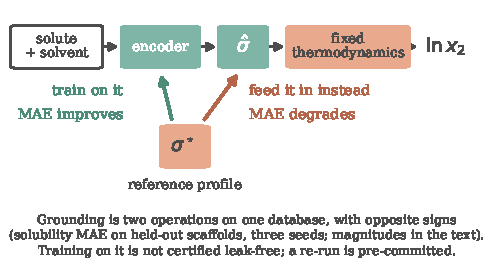
\includegraphics[width=\linewidth,height=1.7in,keepaspectratio]{figs/fig_toc.pdf}
\end{tocentry}

\begin{abstract}
Physics-informed predictors combine learned physical quantities through a fixed thermodynamic
relation. The arrangement is attractive because a prediction made through named quantities can be
audited, and because a better value for one of them can be looked up and supplied without
retraining. We ask whether the values such a network places in the slot of a physical quantity are
that quantity. The system is a graph network supplying the $\sigma$-profile consumed by COSMO-SAC
to predict the solubility of solids, and every measurement is reported against a control. Solubility
data do not determine the quantities the relation composes. The network places screening-charge
density where quantum chemistry places none, concentrating in the windows that activate the model's
hydrogen-bonding term, and the output layer is not the cause. A molecule's profile depends on
whether it enters as solute or as solvent, so the model does not return the reference state. The
intermediate does not decompose: replacing part of it with reference values is frequently worse
than replacing none. Supplying the reference profile improves the activity coefficients the profile
exists to produce and degrades the solubility predicted from them.
\end{abstract}

\maketitle

\section{Introduction}
\label{sec:intro}

How much of a solid dissolves in a given liquid decides whether a drug is formulated as a tablet or
an injection, which solvent a crystallisation runs in, and how a product is purified. Each value is
measured one solute, one solvent and one temperature at a time, so most combinations of industrial
interest have never been measured, and a laboratory that needs one is choosing between running an
experiment and trusting a prediction.

Predictors divide by how much physical structure they impose. A direct model regresses solubility
from descriptors or from a representation learned off the molecular graph, and on extrapolation to
unseen solutes the direct models lead; FastSolv \cite{osanloo2024} reports the lowest errors
on that task. What such a model returns is a single number, silent about which part of the
chemistry produced it. A physics-informed model instead predicts the quantities the physical
picture names: an activity coefficient for the solute--solvent interaction, a melting temperature
and an enthalpy of fusion for the crystal. A fixed thermodynamic relation then combines them.
SolProp \cite{vermeire2022solprop} assembles such a cycle from separately learned components. The fixed relation costs accuracy and buys three things. A prediction made
through it can be taken apart, because each intermediate is a quantity chemists tabulate on its
own. Each intermediate can be supervised against reference data that a direct regressor has no way
to use. And the relation is itself a prior, asserting for free what a purely statistical model
would have to learn from data it does not have, which is the situation whenever the molecule in
question is unlike anything in the training set.

Among those intermediates the $\sigma$-profile is the one most often learned. In the
conductor-like screening model for real solvents and in its segment-activity reformulation
COSMO-SAC \cite{lin2002}, a molecule enters the thermodynamics only through the distribution of
screening-charge density over its cavity surface: how much of that surface carries charge density
of each value. The distribution comes from a quantum-chemical calculation with a continuum
solvation treatment and is tabulated once per molecule \cite{mullins2006}, after which a
closed-form segment-activity expression consumes it and knows nothing else about the compound.
That makes it an unusually clean target for learning. It is a fixed-length vector, it is tabulated
for thousands of molecules, and supplying it from structure removes the only expensive step in the
pipeline. Group-contribution schemes supplied it first \cite{mu2007gc,mu2009gc}, and learned
predictors followed, taking the profile from a line notation or a molecular graph
\cite{kang2022surrogate,chen2021transformer,zhang2022mpnn}. How far the tabulated reference itself
moves with the quantum chemistry and solvation treatment behind it is a separate and live question
\cite{salih2025sigma}. An older line regresses an \emph{apparent} profile from phase-equilibrium
data instead \cite{islam2015apparent}, which is the pre-neural form of the effective profile
measured here.

All of this rests on a premise rarely written down, because it reads as though it needs no writing.
If the quantity in the slot is a $\sigma$-profile, then a network that fills the slot has learned a
$\sigma$-profile. The usual consequences follow: it can be read as chemistry, and it can be
compared against tabulation. The strongest consequence is that a better value can be looked up and
handed back to the model without retraining, and the prediction should improve. The premise is what makes the
intermediate worth having, since it is the difference between a physical model and an elaborate
parameterisation. The recent literature states it in close to those words. The physics-embedded
phase-equilibrium model closest to the work reported here argues that its intermediate carries
clear physical significance because it appears directly in the thermodynamic formulation
\cite{yang2025tennet}. That argument is about the equations. Whether the values a network places in
the slot are the physical quantity is a different question, and it takes a different kind of
answer.

There is reason to expect that they are not. In machine learning the same construction is called a
concept bottleneck \cite{koh2020cbm}. A network is required to predict named, human-meaningful
concepts, and the target is predicted from those concepts alone, in the expectation that the
prediction becomes interpretable and that intervening on a concept behaves as its name implies. The
concepts leak. A bottleneck trained end to end carries information its labels do not name, the
downstream model reads it for more than its nominal content, and both the interpretation and the
interventions then fail in ways the names do not predict
\cite{margeloiu2021,mahinpei2021,havasi2022}. A $\sigma$-profile head inside a fixed closure is
that construction with a thermodynamic decoder in place of a learned one, and it differs in one
respect that matters: the concept has a ground truth. A $\sigma$-profile is not a human label but a
computable quantity, so leakage can be measured against the quantity itself rather than inferred
from downstream behaviour. The structural reason for leakage is also sharper here. A solubility
measurement constrains the \emph{composition} of the intermediate with the fixed relation, not the
intermediate itself. Where different intermediates compose to the same target, the data cannot
choose between them, and the combinations it leaves undetermined are where a flexible network is
free to move. This is the familiar predicament of a model whose parameters are weakly constrained
by its observables \cite{gutenkunst2007,transtrum2015,raue2009}, compounded by calibration against
a relation that is itself only approximate \cite{kennedy2001,brynjarsdottir2014}.

The literature has, without saying so, already taken a position on this. In the physics-embedded
model nearest to the present work, the $\sigma$-profile predictor is trained against
quantum-chemical profiles and then held fixed. At the fine-tuning stage every component and layer
is frozen except the output head of the segment-activity network, so no gradient from the
experimental phase-equilibrium data reaches the intermediate \cite{yang2025tennet}. At the
other end of the same axis sit models that learn a thermodynamic potential from equilibrium
compositions with no supervision on the intermediate at all, and models that dispense with the
named intermediate and impose the thermodynamics in the architecture instead
\cite{specht2024hanna}. The axis is a design choice about how far the intermediate is allowed to
move under the target's gradient. It is made differently in nearly every paper and argued for in
none of them. The pipeline studied here sits in the middle by construction: its $\sigma$-profile
head is supervised against the same tabulated reference, and the closure's gradient also reaches
it. That is what makes it a place where the cost of the choice can be read.

This paper asks what a network puts in that slot, on one pipeline and one intermediate, and reports
a battery of measurements rather than a model. The first asks whether solubility determines the
profile at all, and answers through the curvature of the likelihood in the directions the closure
exposes. The second asks whether the head uses the freedom the first one finds, and where on the
charge-density axis it goes. The third asks whether the architecture is responsible, by testing
whether the output layer that cannot represent an exact zero is the reason the learned profile
carries charge density where the reference carries none. The fourth asks whether the resulting
profile still respects the reference state, that is whether a molecule dissolved in itself is
predicted to be ideal. The fifth asks what the misfit costs the closure and where on the grid that
cost is located. The sixth asks whether the intermediate decomposes at all, by replacing parts of
the learned profile with the reference and asking whether the parts add up. The last asks when
supplying a faithful intermediate helps, using a second and better-specified closure for contrast.
Each test is stated with the result that would refute its reading before it is run, because several
of them return negatives, and a negative that is wrong closes a direction instead of correcting
it.

Three things the paper does not claim. It does not report a more accurate solubility model. On the
scaffold-disjoint split used throughout, the physics path trails a matched direct control in the
seed mean, and both sit near a random-forest baseline. Both are also well behind the external state
of the art on extrapolation to new solutes, and the absolute errors are within reach of the
disagreement between independent measurements of the same system. It is not a benchmark against any published
model, because no published model was retrained here; the comparison with prior art is a comparison
of design choices and of what each design leaves unmeasured. And it does not show that learning a
$\sigma$-profile is a poor design. It shows what has to be measured before the learned profile is
read as one.


\section{The system under study}
\label{sec:system}

\subsection{The relation being closed}

The solubility of a crystalline solid in a liquid follows from a balance between two quantities.
Breaking the crystal costs an amount set by the melting temperature $T_m$ and the enthalpy of
fusion $\Delta H_{\mathrm{fus}}$; mixing the freed molecules into the solvent is governed by the
activity coefficient $\gamma_2$ of the solute in that solvent. For an ideal solution the two
combine into the mole fraction at saturation,
%
\begin{equation}
\ln x_2 \;=\; -\,\Phi(T) \;-\; \ln \gamma_2 ,
\qquad
\Phi(T) \;=\; \frac{\Delta H_{\mathrm{fus}}}{R}\!\left(\frac{1}{T} - \frac{1}{T_m}\right),
\label{eq:sle}
\end{equation}
%
with $R$ the gas constant. The first term is the crystal contribution and carries no information
about the solvent; the second is where the chemistry of the mixture enters. Because $\gamma_2$
itself depends on $x_2$, equation~\eqref{eq:sle} is solved rather than evaluated.

COSMO-SAC \cite{lin2002} supplies $\gamma_2$. It represents each molecule by its $\sigma$-profile:
the area of the molecular cavity surface carrying screening-charge density $\sigma$, discretised
onto a fixed grid of $51$ bins spanning roughly $\pm 0.025\,e\,\mathrm{\AA}^{-2}$. A molecule's
identity enters the model through this vector and through the total cavity area; nothing else about
the compound is used. Segments exchange with a common pool, and a self-consistent calculation
returns a segment activity coefficient for each bin, from which the molecular activity coefficient
follows. The exchange energy contains a term that switches on only for segments beyond a threshold
$\sigma_{\mathrm{hb}}$ in magnitude, which is how the model represents hydrogen bonding; a segment
qualifies by its charge density alone, with no reference to which atom carries it. That threshold
divides the charge-density axis into a core and two outer windows, and the division recurs
throughout what follows.

\subsection{The network that supplies the profile}

A graph neural network reads the solute and the solvent and produces, for each, a $\sigma$-profile
and a cavity area; these are passed to the COSMO-SAC calculation and to the solver for
equation~\eqref{eq:sle}. A second head predicts the crystal properties $T_m$ and
$\Delta H_{\mathrm{fus}}$ that enter $\Phi(T)$. The profile head is a feed-forward network on the per-molecule representation, ending in a normalised, non-negative vector of $51$ bins. The same head serves both roles, but reads a role-dependent representation, so a compound receives one profile as solute and another as solvent.

The head is trained in two ways at once, and this is the property that makes the pipeline suitable
for the present question. It is supervised directly against tabulated reference profiles, as a
predictor of those profiles would be. It is also trained through the thermodynamic relation, so
the gradient of the solubility loss reaches it. The nearest prior model instead supervises its
profile predictor externally and then freezes it, so that no gradient from the phase-equilibrium
data reaches the intermediate \cite{yang2025tennet}. The pipeline studied here therefore occupies
the position where both influences act, which is where their relative effect can be read.

\subsection{Reference profiles, data and arms}

Reference $\sigma$-profiles are taken from the VT-2005 tabulation \cite{mullins2006}, computed by
quantum chemistry with a continuum solvation treatment. Throughout, ``reference'' means a value
from that table, and departures are measured against it. How far the tabulation itself depends on
the underlying electronic structure method is a separate question \cite{salih2025sigma} and is not
at issue here, since every comparison in this work uses one table.

Solubility data are drawn from a curated compilation of measured solid solubilities
\cite{krasnov2025bigsoldb}, split so that no scaffold \cite{bemis1996} appears in both training and
test sets, which is the harder of the two standard settings and the one relevant to new compounds.
Infinite-dilution activity coefficients used to score the closure directly come from an independent
compilation. All results below are reported over five training seeds; the arms differ only in the
seed, so the spread across them is the natural scale against which any effect must be read.
Architectural details, hyperparameters, the construction of the splits and the auxiliary
supervision streams are given in the Supporting Information.

\subsection{How the measurements are read}

Each measurement in Section~\ref{sec:results} is a contrast, and each is reported against a control
chosen so that it would fire if the instrument responded to something other than the intended
effect. Where a quantity is compared with a reference table, the control is the same quantity
computed on profiles that carry the same total area but no chemistry. Where part of a profile is
replaced, the control is a part of the same size chosen at random. Where an effect is attributed to
training, the control is an untrained network of the same architecture. The reading rule for each
measurement, together with the result that would refute it, was fixed before the measurement was
made; the rules and their outcomes are listed in the Supporting Information. Table~\ref{tab:battery}
collects every test with the control beside it, because a result of this kind is not interpretable
without one.


\begin{figure*}[t]
\centering
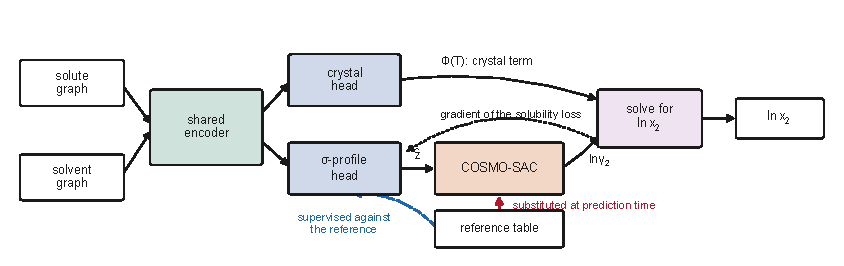
\includegraphics[width=\linewidth]{figs/fig_pipeline.pdf}
\caption{The pipeline. A shared encoder reads the solute and solvent graphs; one head supplies the
crystal term of equation~\eqref{eq:sle} and another the $\sigma$-profile $\hat{z}$ consumed by
COSMO-SAC. The profile head is supervised against the reference table and also receives the
gradient of the solubility loss. At prediction time the reference profile can replace the learned
one.}
\label{fig:pipeline}
\end{figure*}

% СГЕНЕРИРОВАНО scripts/analysis/make_battery_table_tex.py -- НЕ ПРАВИТЬ РУКАМИ.
% Каждое число читается из депозита по ключу; правка здесь разойдётся с артефактом молча.
\begin{table*}[t]
\centering
\small
\caption{The diagnostic battery. Each test is read against the null named beside it; a result without its null is not a result. Numbers are medians over five training seeds unless a range is given.}
\label{tab:battery}
\begin{tabular}{@{}p{0.19\linewidth}p{0.27\linewidth}p{0.27\linewidth}p{0.21\linewidth}@{}}
\toprule
Question & Instrument, and the null it is read against & Result & Reading \\
\midrule
Does solubility determine the factors it composes? & Fisher information of the four-parameter fit; Cram\'er--Rao bound on the enthalpy of fusion, against the same bound with external labels supplied & condition number $2.3\times10^{5}$; bound $\pm20$\,kJ\,mol$^{-1}$, falling to $\pm1.7$ with the labels & No. The crystal enthalpy is collinear with the activity's temperature slope. \\
\addlinespace[2pt]

Does the head use the freedom? & residual of learned minus reference profile by charge-density window, 71 molecules, against each window's share of surface area & donor window $4.0\times$, acceptor $2.0\times$, nonpolar core $0.88\times$ & Yes, and into the windows the hydrogen-bonding term reads. \\
\addlinespace[2pt]

Is the output layer responsible? & mass in bins where the reference is exactly zero, against the smallest bin the same head reaches anywhere and against an untrained head & head reaches $10^{-11}$; 34--51\% of those bins already below $10^{-5}$; pedestal 0.02--0.03 against 0.57 untrained & No. The pedestal is learned. 58\% of reference cells are exactly zero. \\
\addlinespace[2pt]

Is the reference state preserved? & activity of a molecule in itself, against the one-profile control that must return zero identically & control $0$ exactly; median $|\ln\gamma|$ 0.012--0.044, largest 0.80 & No. A molecule's two role profiles do not coincide. \\
\addlinespace[2pt]

What does misplaced mass cost, and where? & mean $|\Delta\ln\gamma|$ from moving a fixed mass into each bin, against random profiles of the same area & edge-to-core ratio $21\times$ and $15\times$ on the two row sets, against $1.6\times$ for random profiles & Strongly non-uniform, with a step at the bonding threshold. \\
\addlinespace[2pt]

Does the intermediate decompose? & reference shape substituted into part of the grid, against a randomly chosen part of the same size & the whole shape helps on 5 of 5 seeds; a random third is worse than the fully learned profile in 94\% of draws & No. The parts do not add, so per-bin attribution is undefined. \\
\addlinespace[2pt]

Where does the error that reaches the closure live? & reference shape in the bins where it is nonzero, against exact zeros in the bins where it is zero & $+89\%$ of the gap recovered against $-9\%$ & In the magnitude of the occupied bins, not in the pedestal. \\
\addlinespace[2pt]
\bottomrule
\end{tabular}
\end{table*}


\section{Results}
\label{sec:results}

Table~\ref{tab:battery} lists every measurement reported below together with the control it is read
against. The order follows the question rather than the chronology: first whether the data
determine the internal quantity at all, then what the network does with the freedom that remains,
then what that costs the thermodynamics.

\subsection{The observable determines two of fifty directions of the profile}
\label{sec:ident}

A $\sigma$-profile is a point in a $51$-dimensional space, and normalisation fixes one direction, so
a profile can move in $50$. The question is how many of those the closure exposes. For each
solvent we collected the rows in which it appears, differentiated the predicted activity
coefficient with respect to its profile, and took the spectrum of the resulting information matrix.
Over $25$ solvents and five seeds, the number of directions carrying $99\%$ of the information is
$2$, with a range of $1$ to $5$; the median condition number is $1.4\times10^{33}$. The remaining
directions are not merely poorly determined. They are flat to numerical precision, so a profile can
move along them without changing any prediction the closure makes.

The same calculation on random profiles of equal area returns the same count. The deficiency is
therefore structural, a property of the exchange kernel and of the diversity of partners available,
rather than something the trained head produced. That is the stronger of the two readings: it holds
wherever the profile is linearised, not only at the point this network happens to occupy.

The crystal term is underdetermined in the same way and for a reason that is easier to picture. The
enthalpy of fusion and the temperature slope of the activity coefficient both enter
equation~\eqref{eq:sle} through $1/T$, so a fit can trade one against the other. For the
four-parameter fit the condition number of the information matrix is $2.3\times10^{5}$, and no
estimator can determine the enthalpy of fusion from a solubility series to better than about
$\pm20$~kJ\,mol$^{-1}$, which is wider than the range the quantity takes across these compounds.
Supplying the melting temperature and the enthalpy of fusion as independent labels reduces that
bound to $\pm1.7$~kJ\,mol$^{-1}$.

What the network places in the undetermined directions is not decided by the data. The rest of this
section measures what it places there.

\subsection{The network places charge density where the reference carries none}
\label{sec:windows}

The reference tabulation is sparse. A molecule with no hydrogen-bond donor is tabulated with no
cavity surface carrying donor-side charge density, and $58\%$ of all reference cells across the
compounds examined here are exactly zero, a median of $29$ bins of $51$ per molecule.

The learned profiles are not sparse anywhere. Figure~\ref{fig:windows} shows the donor-window area
for sixteen common solvents. Twelve of the sixteen are exactly empty in that window in the
reference; all sixteen carry area there in the learned profile, between $0.1\%$ and $5.2\%$ of the
molecule's surface. The hydrogen-bonding term reads that area regardless of how small it is,
because a segment qualifies for the term by its charge density alone.

Where the misfit lands is not uniform across the charge-density axis. Take the residual between the
learned and the reference profile over the $71$ molecules that appear in a labelled test row, and
express it relative to the share of surface area each window holds. The donor window is then
over-represented by a factor of $4.0$ and the acceptor window by $2.0$, while the nonpolar core is
under-represented at $0.88$. The profiles a molecule receives as solvent give $3.8$, $2.0$ and
$0.89$ for the same three windows, so the orientation of the displacement does not depend on which
role the molecule plays. The network's departure from the tabulation concentrates in the regions
that switch on the model's hydrogen-bonding term and thins in the region that does not.

\subsection{The output layer is not the cause}
\label{sec:pedestal}

An obvious explanation is architectural. The head ends in a normalisation that cannot return an
exact zero, so a profile that should be empty in a bin will instead be slightly populated there,
and the defect would be an artefact of the parameterisation. The explanation is testable, and it
fails.

Figure~\ref{fig:pedestal}a shows, for every bin in which the reference is exactly zero, how much
mass the trained head places there. The distribution reaches $1.0\times10^{-11}$, and between
$34\%$ and $51\%$ of those bins already lie below $10^{-5}$. A layer that can reach $10^{-11}$ is
not what holds the remaining bins at $10^{-5}$. Figure~\ref{fig:pedestal}b makes the same point
from the other direction. An untrained network of the same architecture places a median of $0.571$
of the profile's mass in the bins where the reference is empty; after training the figure is
$0.022\pm0.004$ over five seeds and both roles. The residual population is something training
arrives at, not something the parameterisation imposes.

The two roles agree. The pedestal is $0.024\pm0.004$ on the profiles a molecule receives as solute
and $0.020\pm0.003$ on those it receives as solvent, a difference of $0.004$ against a
seed-to-seed spread of the same size. This measurement and the one in
Section~\ref{sec:windows} therefore hold separately for each of the two profiles a molecule is
given, and do not depend on the fact that it is given two.

The point extends beyond the present pipeline. A recent physics-embedded model uses a rectified
output with the same normalisation and can therefore emit exact zeros \cite{yang2025tennet}. The
measurement above indicates that the difference between the two output layers is not what decides
whether a learned profile resembles the tabulated one.

\subsection{A molecule is not ideal in itself}
\label{sec:refstate}

Any activity coefficient model must return unity for a pure component, since a molecule surrounded
by copies of itself is in its reference state by definition. In COSMO-SAC the property holds
identically: the residual term is a difference between a segment's activity in the mixture and in
the pure compound, and the two coincide when one profile is used on both sides. Supplying a single
profile to both sides returns exactly zero here, which confirms that the implementation carries the
property.

The pipeline does not. Because the head reads a role-dependent representation, a compound receives
one profile as solute and a different one as solvent, so pairing a molecule with itself pairs two
different profiles. The median departure from ideality is between $0.012$ and $0.044$ in
$\ln\gamma$ across the five seeds, the ninety-fifth percentile between $0.09$ and $0.34$, and the
largest single value is $0.80$. The violation belongs to the learned intermediate rather than to
the thermodynamic relation. It is also invisible in any evaluation that never pairs a compound with
itself, which is every evaluation on solubility or on mixture data.

\subsection{What misplaced density costs, and where}
\label{sec:cost}

The preceding measurements establish that density sits where the reference says it should not. They
do not say what that costs, and the cost is not uniform. Figure~\ref{fig:costmap}a reports, for
each bin, the mean change in the predicted activity coefficient produced by moving a fixed amount
of mass from the core into that bin. Moving mass within the core is almost free. Moving the same
mass into the outer windows costs $21$ times as much as a median over seeds, with a range of $21$
to $30$; computed over the rows used for scoring rather than for training the ratio is $15$, with a
range of $13$ to $25$. Random profiles of the same total area give $1.6$ and $1.5$, so the
structure reflects the chemistry of the exchange rather than the geometry of the grid.

The cost does not grow smoothly with distance along the axis. It is flat across the core, rises
steeply as the hydrogen-bonding threshold is crossed, and then saturates. Once mass is inside the
bonding region, pushing it further out changes the prediction comparatively little. The consequence
is shown in Figure~\ref{fig:costmap}b. Reading the measured cost as a potential and taking its
gradient gives the weight under which the usual transport distance between two profiles would price
their difference correctly, and that weight peaks at the boundary rather than deep in the outer
window. A treatment that weighted the far corner most heavily, which is what the geometry of the
grid would suggest, would weight the wrong place.

\subsection{The intermediate does not decompose}
\label{sec:nonadditive}

If the learned profile were a $\sigma$-profile carrying a per-bin error, then correcting part of it
should help in proportion to the part corrected. It does not. Replacing the learned shape with the
reference shape over the whole grid improves the predicted activity coefficients on all five seeds.
Replacing it over a randomly chosen third of the bins makes the prediction worse than leaving the
profile entirely alone in $20\%$ of draws, taken over twenty random thirds at each of five seeds and
ranging from $5\%$ to $30\%$ by seed. Recovery of the gap across those draws runs from $-213\%$ to
$+152\%$.

A profile assembled from correct values in some bins and learned values in the rest is not
intermediate between the two. The segment-activity calculation is a self-consistent solution over
the whole distribution, so an internally inconsistent profile can sit far from both of the profiles
it was built from. Two things follow. The first is methodological: the share of the error
attributable to any subset of bins is not defined on this surface, so an analysis that partitions
the grid and attributes error to the parts cannot be carried out, whatever the partition. The
second concerns the premise under test. Partial correctness of the intermediate is not partially
useful, and is frequently worse than consistent incorrectness.

\subsection{The error that reaches the thermodynamics is in the occupied bins}
\label{sec:attribution}

One partition is well posed, because both of its parts are substituted in full: the bins where the
reference is nonzero, and the bins where it is zero. Figure~\ref{fig:attribution}a reports both.
Supplying the reference values in the bins the reference occupies recovers $89\%$ of the gap
between the learned and the reference profile, positive on all five seeds and ranging from $68\%$
to $109\%$. Setting exact zeros in the bins the reference leaves empty recovers $-9\%$ on average,
with a per-seed range from $-36\%$ to $+34\%$, and the result sits inside the spread of a control
that zeroes the same number of randomly chosen cells.

The spurious density is therefore not what the thermodynamics responds to. The error that
propagates through the closure lives in the magnitude of the profile where the profile is
populated. The cost map of Section~\ref{sec:cost} does not localise this error either.
Figure~\ref{fig:attribution}b shows that substituting the reference into the third of the grid the
closure is most sensitive to recovers no more of the gap than substituting into a randomly chosen
third, and that the sign varies across seeds. Sensitivity per unit of displaced mass and total
contribution to the error are different quantities, and the core carries most of the mass.

The profile's shape and the molecule's cavity area, which COSMO-SAC consumes as a separate scalar,
split the gap unevenly. Replacing the whole shape while keeping the learned area moves the mean
error from $1.75$ to $1.08$, against $0.76$ when the reference profile is supplied with its own
area, so the shape accounts for $0.68$ of the gap and the area for the rest. This is a
decomposition of two full substitutions rather than an attribution over bins, and is not subject to
the objection raised in Section~\ref{sec:nonadditive}.

\subsection{Supplying the reference improves one quantity and degrades the other}
\label{sec:twosided}

The substitution the premise licenses can be scored on two quantities at once: the activity
coefficient the profile exists to produce, and the solubility the pipeline is built to predict.
Both are measured on the same checkpoints.

On the activity coefficients, replacing the learned profiles with the reference profiles moves the
mean absolute deviation from $1.751\pm0.063$ to $0.765$, an improvement on every one of the five
seeds and more than fourteen times the seed-to-seed spread of the arm. On the solubility, the same
replacement at prediction time moves the error in the opposite direction, by
$0.431\pm0.044$ in mean absolute error over the $5274$ test rows in which a reference profile was
available for the solvent, with per-seed values of $0.456$, $0.381$ and $0.457$.

The control is internal to the same comparison. No reference profile exists for either component in $37$ test
rows, so nothing is substituted in them, and across those rows the two arms differ by at most
$4\times10^{-6}$ in mean absolute error. The effect is therefore carried by the rows in
which the substitution actually happened, and not by any difference in how the two arms were
scored. The substitution is a solvent-side substitution throughout: of the $147$ distinct solutes
in the test rows only seven are tabulated, so no row exists in which the solute profile alone is
replaced. What is reported is what the available reference data permit, and the solvent channel is
where the comparison lives.

The two directions are the result this work was undertaken to obtain. A better value for the
internal quantity makes the thermodynamic model it feeds more accurate and makes the pipeline less
accurate.


\begin{figure*}[t]
\centering
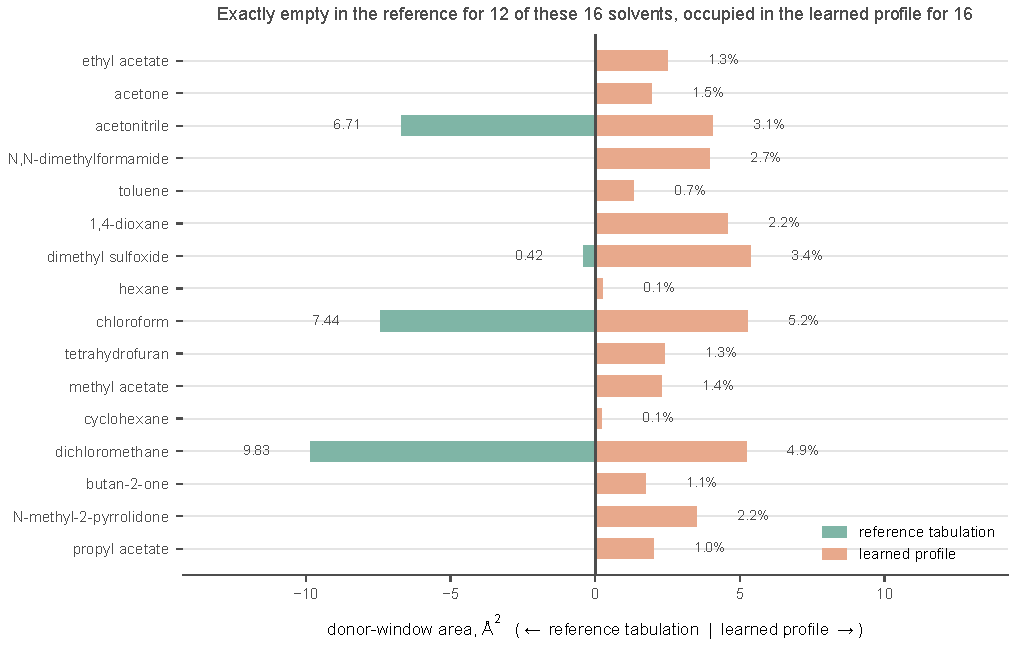
\includegraphics[width=\linewidth]{figs/fig_donor_window.pdf}
\caption{Donor-window area for sixteen solvents in the reference tabulation (left) and in the
learned profile (right). Percentages give that window's share of the molecule's cavity surface in
the learned profile.}
\label{fig:windows}
\end{figure*}

\begin{figure*}[t]
\centering
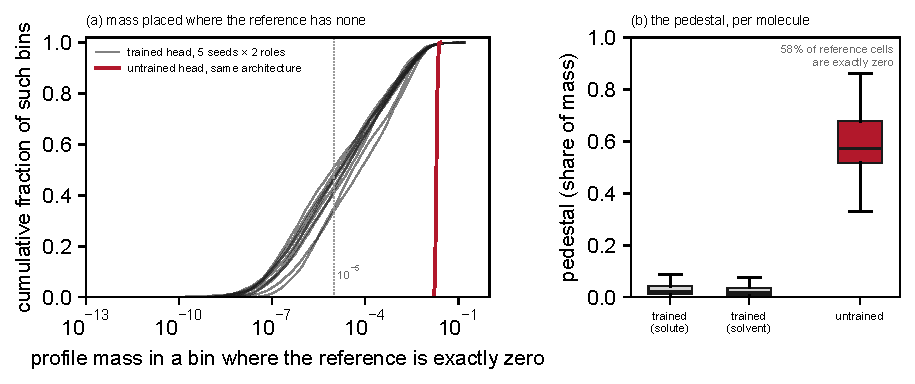
\includegraphics[width=\linewidth]{figs/fig_pedestal_learned.pdf}
\caption{(a) Cumulative distribution of the profile mass placed in bins where the reference is
exactly zero, for five seeds in both roles and for an untrained network of the same architecture.
(b) The same mass summed over each molecule.}
\label{fig:pedestal}
\end{figure*}

\begin{figure}[t]
\centering
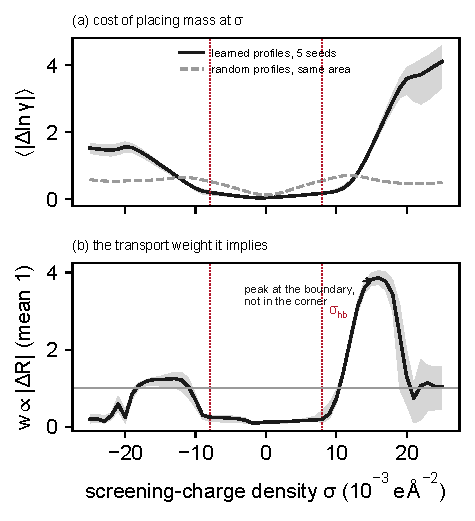
\includegraphics[width=\linewidth]{figs/fig_cost_map.pdf}
\caption{(a) Mean change in the predicted activity coefficient produced by moving a fixed mass from
the core into each bin, for five seeds (band) and for random profiles of the same total area.
(b) The gradient of that cost, normalised to mean one. Dotted lines mark
$\pm\sigma_{\mathrm{hb}}$.}
\label{fig:costmap}
\end{figure}

\begin{figure*}[t]
\centering
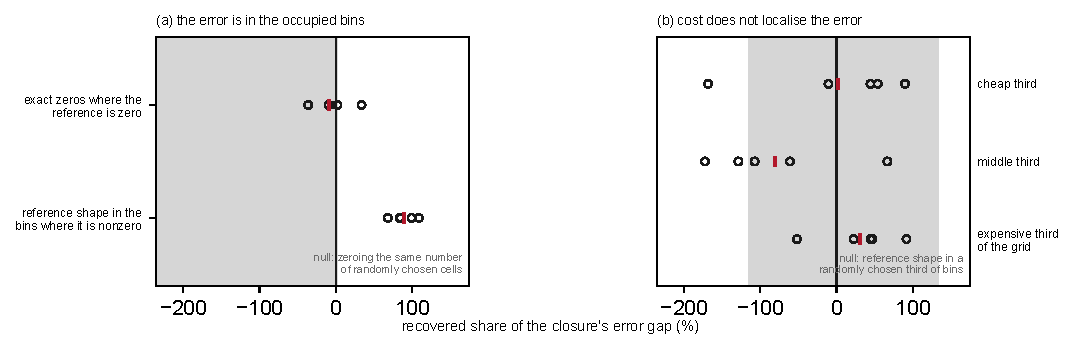
\includegraphics[width=\linewidth]{figs/fig_attribution.pdf}
\caption{Share of the gap between the learned and the reference profile recovered in the predicted
activity coefficients, one circle per seed and a bar at the mean. (a) Reference values supplied in
the bins where the reference is nonzero, and exact zeros in the bins where it is zero.
(b) Reference values supplied in thirds of the grid ordered by the cost of
Figure~\ref{fig:costmap}. The shaded band is the central $90\%$ of the control named in each
panel.}
\label{fig:attribution}
\end{figure*}

\section{Discussion}
\label{sec:discussion}

The measurements describe a quantity that occupies the place of a $\sigma$-profile without being
one. It is sparse where the reference is dense and populated where the reference is empty. It depends on the role the molecule plays in the pair, so the model it feeds does not return the reference state. And it does not decompose, so the familiar move of correcting part of it and expecting part of the benefit is unavailable.

The sharpest statement of the situation is a contrast between two substitutions of the same
values. Supplying the reference profile improves the quantity the profile exists to produce: the
predicted activity coefficients move most of the way toward the measured ones, on every seed. The
same substitution degrades the solubility the pipeline is built to predict. Both facts are measured
on the same checkpoints and the same compounds. Taken together they say that the downstream parts of the model have adapted to the profile the network supplies rather than to the one the physical argument names. Handing the model a physically better value therefore moves it away from the operating point it was fitted at. This is the behaviour the concept-bottleneck literature reports
for learned concepts in general \cite{koh2020cbm,margeloiu2021}, arrived at here through a
thermodynamic decoder and, because the concept has a computable ground truth, measured against the
concept itself rather than inferred from how interventions behave.

It follows that the assumption set out in the Introduction is not a property of physics-informed
models as such but a property of how the internal quantity is trained. The design choice that
matters is whether the gradient of the target reaches the intermediate. Where it does not, as in a
model whose profile predictor is supervised externally and then frozen \cite{yang2025tennet}, the
intermediate should remain what it is named after to within its own fit error, and substitution
should be a sensible operation. That expectation is not tested here, since the model in question
was not retrained. Where it does, the intermediate becomes a free internal coordinate that happens
to be initialised and regularised toward a physical quantity, and the operations the physical
reading licenses stop being safe. The present pipeline sits between the two, with both influences
acting, and the measurements show which one wins.

For practice this suggests a different division of labour than the one the literature has settled
into. If the internal quantity is to be read as chemistry, exchanged with tabulated values, or audited against reference data, it should be supervised against that reference and then held fixed. The capacity needed to fit the data belongs somewhere that makes no physical claim.
If instead the intermediate is allowed to move under the target's gradient, the gain in accuracy
is real but the physical reading has to be dropped, and with it the argument that recommends these
models over direct regression in the first place. What is not available is to train the
intermediate end to end and retain the interpretation, which is the position most of this
literature currently occupies.

Three measurements in the battery are worth separating from the rest because each removes an
explanation that would otherwise be reached for. The output layer is not responsible for the
spurious density: the same head reaches values six orders of magnitude smaller elsewhere in the
same profile. The cost map does not localise the error: the bins the closure is most sensitive to account for no more of the gap than a randomly chosen third. Sensitivity is measured per unit of displaced mass, and most of the mass sits in the insensitive core. And the spurious
density in the empty bins, the most visible defect and the one easiest to describe, is not what the
thermodynamics responds to; the error that propagates is in the magnitude of the profile where the
profile is populated.

The finding is conditional on the fixed relation being an adequate description of the chemistry it
is applied to. Where a relation is well specified for its domain, supplying it with more accurate inputs behaves as the physical reading predicts. A second system, in which a linear free-energy relation stands in for the closure and its adequacy varies by chemical stratum, separates in that way; it is reported in the Supporting Information. The result here should therefore be read as a
statement about an intermediate trained through an approximate closure, which is the common case,
rather than as an argument against building physics into a model.

\section{Limitations}
\label{sec:limitations}

The evidence comes from one pipeline, one closure and one reference tabulation. Every departure reported above is measured against the VT-2005 table. How far that table itself moves with the electronic structure and solvation treatment behind it is a separate question \cite{salih2025sigma}. A different tabulation would shift the reference against which the learned profile is scored, but not the comparisons between arms, which all use one table.

A zero in that table is a tabulated zero. The $\sigma$-profile is built by binning a finite set of
surface segments, so a bin can be empty because no segment of the molecule falls in it as well as
because the molecule cannot carry charge density of that value. The distinction does not affect the
comparisons reported here, all of which treat the tabulation as the reference. It does bound how
strongly the finding may be stated: what is measured is a departure from the tabulated
distribution, not a departure from a proven absence of density.

The profile head reads a role-dependent representation, so a molecule receives two profiles. That
is a choice made in this pipeline, and a reader is entitled to ask whether the defects reported
above are consequences of it. For two of them the question is settled by measurement. The window
displacement of Section~\ref{sec:windows} and the residual population of
Section~\ref{sec:pedestal} are the same on each of the two profiles taken separately, with the
difference between roles no larger than the spread across seeds. The violation of the reference
state in Section~\ref{sec:refstate} is a direct consequence of the choice and would disappear under
a role-independent head, at a cost in accuracy that is not measured here. The non-additivity of
Section~\ref{sec:nonadditive} is a property of the segment-activity calculation rather than of the
head, since it concerns how the closure responds to an internally inconsistent profile. An arm
trained with a role-independent head would settle the remaining cases directly, and has not been
run.

Equation~\eqref{eq:sle} omits the heat-capacity difference between the solid and the subcooled
liquid, as is usual. Where the temperature lies far below the melting point that term is not
negligible, and it adds a further source of indeterminacy to the crystal contribution beyond the
collinearity reported in Section~\ref{sec:ident}.

The activity coefficients used to score the closure are at infinite dilution, while the solubility
the pipeline predicts is a finite mole fraction at saturation. The two are the same functional of
the same profiles evaluated at different compositions. The comparison in
Section~\ref{sec:twosided} therefore reports the direction of the substitution's effect on each,
not a single error carried between them.

This work does not report a more accurate solubility model. On the scaffold-disjoint split used
throughout, the physics path trails a matched direct control sharing the same encoder in the mean
over seeds, and both sit near a random-forest baseline. Both are well behind the leading direct
models on extrapolation to new solutes \cite{osanloo2024}, and absolute errors are within reach of
the disagreement between independent measurements of the same system. No published model was
retrained here, so the comparison with prior work is a comparison of design choices rather than of
performance.

Results are reported over five training seeds, and for some quantities that is not enough. The cost of the spurious density, expressed in the error of the predicted activity coefficients, varies across seeds by several times the spread of the arms themselves. Its sign is therefore not determined by the present evidence. What is determined is that it is not large and positive. The
asymmetry of the cost map between the two sides of the charge-density axis depends on which set of
molecule pairs it is computed over, and is reported for both.

The closure is the 2002 formulation of COSMO-SAC with a single hydrogen-bonding term, run without
the combinatorial contribution. That term needs molar volumes, which the source database carries
but the extracted table used here does not, and which the network could supply with a second scalar
head beside the one that already predicts cavity area. Its omission is a choice made when the table
was extracted rather than a constraint. The term vanishes for a pair of a molecule with itself, so
Section~\ref{sec:refstate} is unaffected; it would change the magnitudes in
Sections~\ref{sec:cost} and~\ref{sec:attribution}, where the size of the effect is the result. Later
formulations split the hydrogen-bonding term by segment type and would change where on the
charge-density axis the cost steps, though not the existence of a step. The segment calculation is
iterated to a fixed count; the count used at training and at scoring is recorded with each run,
because the two need not agree and the predicted activity coefficients depend on them.

Finally, the measurements concern substitution at prediction time on an intermediate that was
trained through the closure. They do not establish what would happen in a model whose intermediate
is supervised externally and frozen. That design is the one the results recommend, and testing it
requires training such a model rather than measuring this one.

\section{Conclusions}
\label{sec:conclusions}

A network trained inside a fixed thermodynamic relation fills the relation's input slot with values
that are not the physical quantity the slot names. The learned $\sigma$-profile places
screening-charge density where the reference tabulation carries none, concentrating in the windows
that trigger the model's hydrogen-bonding term. It differs depending on whether the molecule is treated as solute or solvent, so a molecule is not predicted to be ideal in itself. And it cannot be corrected in parts: replacing a fraction of it with reference values is often worse than replacing none. The output layer is not the cause, and the error that reaches the thermodynamics
lies in the magnitude of the profile where it is populated rather than in the spurious density
where it should be empty.

Supplying the reference profile improves the activity coefficients the profile exists to produce
and degrades the solubility the pipeline predicts. The interpretation that makes physics-informed
models attractive, that a better value for an internal quantity can be looked up and handed to the
model, holds only where that quantity is supervised externally and shielded from the target's
gradient. Where the intermediate is trained end to end, it is an internal coordinate with a
physical name, and the operations the name licenses should be measured before they are used.


\section*{Author contributions}
\noindent
N.~L. Polomoshnov: Conceptualization, Methodology, Software, Formal analysis, Investigation,
Data curation, Visualization, Writing -- original draft.
A.~V. Rudik: Writing -- review \& editing.

\section*{Funding}
\noindent The study was supported by the Russian Science Foundation, project No.~25-25-00148,
\url{https://rscf.ru/project/25-25-00148/}.

\section*{Notes}
\noindent The authors declare no competing financial interest.

\section*{Acknowledgement}
\noindent Parts of the analysis code and of the manuscript text were drafted with the assistance of
a large language model, under author direction; all reported measurements were produced by code in
the deposited repository and checked by the authors against the deposited artifacts.

\section*{Data and Software Availability}
The analysis code and the intermediate artifacts small enough to version are available at
\url{https://github.com/doctawho42/tgnn-solv} under the MIT licence; the commit the reported
numbers were produced from is recorded in the deposit. Model checkpoints, the processed split and
the per-arm prediction files are deposited in the Zenodo archive
\texttt{10.5281/zenodo.22263434}. The deposit covers the COSMO-SAC arms reported here; weights for
the NRTL variants discussed in the Supporting Information were not retained. Solubility data are
BigSolDB~2.0 \cite{krasnov2025bigsoldb}; reference $\sigma$-profiles are the VT-2005 database
\cite{mullins2006} as redistributed with Ref.~\cite{bell2020cosmosac}; infinite-dilution activity
coefficients are from ThermoML \cite{frenkel2011thermoml}; the acid-dissociation data used in the
Supporting Information are the OPERA compilation \cite{mansouri2019opera}.

\section*{Supporting Information Available}
Architecture and training details; construction of the splits and the auxiliary supervision
streams; the pre-declared reading rule for each measurement with its outcome; the decomposition of
the model's error against what its inputs leave unresolved; and the second system based on a linear
free-energy relation.

\bibliography{references_verified}

\end{document}
